\chapter{Partial Derivatives and Gradients}

This chapter will introduce you to partial derivatives and gradients,
equipping you with the tools to study functions of multiple
variables. We will explore how these concepts provide valuable
insights into optimization, vector calculus, and various fields of
science and engineering.

Partial derivatives come into play when dealing with functions that
depend on multiple variables. Unlike ordinary derivatives that
consider changes along a single variable, partial derivatives focus on
how a function changes concerning each individual variable while
holding the others constant. In essence, partial derivatives measure
the rate of change of a function with respect to one variable while
keeping the other variables fixed.\index{partial derivative}

The notation for a partial derivative of a function $f(x, y, \ldots)$
with respect to a specific variable, say $x$, is denoted as
$\frac{{\partial f}}{{\partial x}}$. Similarly, $\frac{{\partial
    f}}{{\partial y}}$ represents the partial derivative with respect
to $y$, and so on. It is essential to remember that when taking
partial derivatives, we treat the other variables as constants during
the differentiation process.

The gradient is a vector that combines the partial derivatives of a
function. It provides a concise representation of the direction and
magnitude of the steepest ascent or descent of the function. The
gradient vector points in the direction of the greatest rate of
increase of the function. By understanding the gradient, we gain
insights into optimizing functions and finding critical points where
the function reaches maximum or minimum values.\index{gradient}

Throughout this chapter, we will explore the following key topics
related to partial derivatives and gradients:

\begin{itemize}
\item Calculating partial derivatives: We will delve into the
  techniques and rules for computing partial derivatives of various
  functions, including polynomials, exponential functions, and
  trigonometric functions. We will also explore higher-order partial
  derivatives and mixed partial derivatives.

\item Interpreting partial derivatives: Understanding the geometric
  and physical interpretations of partial derivatives is essential. We
  will discuss the notion of tangent planes, directional derivatives,
  and the relationship between partial derivatives and local
  linearity.

\item Gradient vectors and their properties: We will introduce the
  gradient vector and its properties, such as its connection to the
  direction of steepest ascent, its relationship with partial
  derivatives, and how it relates to level curves and level surfaces.

\item Applications of partial derivatives and gradients: We will
  explore various applications of these concepts, including
  optimization problems, constrained optimization, tangent planes,
  linear approximations, and their relevance in fields like physics,
  economics, and engineering.
\end{itemize}

By grasping the concepts of partial derivatives and gradients, you
will unlock a powerful mathematical framework for analyzing and
optimizing functions of multiple variables. These tools will equip you
to tackle advanced calculus problems and gain deeper insights into the
behavior of functions in diverse fields.

\section{Calculating Partial Derivatives}
For a function of two variables, $f(x,y)$, we can take the derivative with 
respect to $x$ or with respect to $y$. These are called the \textit{partial 
derivatives} of $f$.\index{partial derivative} Formally, the partial 
derivatives are defined as:

\begin{mdframed}[style = important, frametitle = {Limit Definition of Partial 
Derivatives}]
$$f_x(x, y) = \lim_{h \to 0} \frac{f(x + h, y) - f(x, y)}{h}$$
$$f_y(x, y) = \lim_{h \to 0} \frac{f(x, y + h) - f(x, y)}{h}$$
\end{mdframed}

Let's consider a polynomial function of two variables: $f(x, y) = 3x^2 + y^3 + 
4xy$. We will use the limit definition to find the partial derivative with 
respect to $x$, then compare this to what we already know about derivatives of 
single-variable functions. Recall that if we can describe a function as a sum of 
two other functions, the derivative of the original function is the same as the 
sum of the derivatives of the other functions. That is, 
$$\text{if } f(x) = g(x) + h(x)$$
$$\text{then } f'(x) = g'(x) + h'(x)$$

Let's then define $r(x, y) = 3x^2$, $s(x, y) = y^3$, and $t(x, y) = 4xy$. And 
so $f(x, y) = r(x, y) + s(x, y) + t(x, y)$, which means $f_x(x, y) = r_x(x, y) 
+ s_x(x, y) + t_x(x, y)$. Then,
$$f_x(x, y) = \lim_{h \to 0} \frac{r(x + h, y) - r(x, y)}{h} + \lim_{h \to 0} 
\frac{s(x + h, y) - s(x, y)}{h} + \lim_{h \to 0} \frac{t(x + h, y) - t(x, y)}{
h}$$
$$= \lim_{h \to 0} \frac{3(x + h)^2 - 3x^2}{h} + \lim_{h \to 0} \frac{y^3 - 
y^3}{h} + \lim_{h \to 0} \frac{4(x + h)y - 4xy}{h}$$
$$= \lim_{h \to 0} \frac{3x^2 + 6xh + h^2 - 3x^2}{h} + 0 + \lim_{h \to 0} 
\frac{4xy + 4hy - 4xy}{h}$$

Notice that $s_x(x, y) = 0$. This term only had $y$, and its derivative with 
respect to $x$ is zero. Continuing, 

$$f_x(x, y) = \lim_{h \to 0} \frac{6xh + h^2}{h} + \lim_{h \to 0} \frac{4hy}{h}
= \lim_{h \to 0} 6x + h + \lim_{h \to 0} 4y$$
$$= 6x + 4y$$

As you can see, $r_x(x, y) = 6x$ and $t_x(x, y) = 4y$. Recall the polynomial 
rule for single derivatives. The derivative of $3x^2$ is $6x$, which is also 
what we see with the partial derivative in this case. What about the other 
term, $4xy$? Well, we know the derivative of $bx$, where $b$ is a constant, is 
$b$. The partial derivative of $4xy$ with respect to $x$ being $4y$ suggests 
the rule for determining partial derivatives:

\begin{mdframed}[style = important, frametitle = {Rule for Finding Partial 
Derivatives of $f(x, y)$}]
\begin{enumerate}
    \item To find the partial derivative with respect to $x$, $f_x$, treat $y$ 
    as a constant and differentiate with respect to $x$.
    \item To find the partial derivative with respect to $y$, $f_y$, treat $x$ 
    as a constant and differentiate with respect to $y$.
\end{enumerate}
\end{mdframed}

Let's check this by predicting $f_y$ and then using the limit definition to 
confirm our prediction. Applying the polynomial rule, we predict that $f_y$ is:
$$f_y(x, y) = 3y^2 + 4x$$

Which we found by treating $x$ as a constant and taking the derivative of each 
term with respect to $y$. Let's see if we get the same result using the limit 
definition of the derivative with respect to $y$:
$$f_y(x, y) = \lim_{h \to 0} \frac{f(x, y + h) - f(x, y)}{h}$$
$$= \lim_{h \to 0} \frac{\left[3x^2 + \left(y + h \right)^3 + 4x \left(y + h 
\right) \right] - \left[ 3x^2 + y^3 + 4xy \right]}{h}$$
$$= \lim_{h \to 0} \frac{3x^2 + y^3 + 3y^2h + 3yh^2 + h^3 + 4xy + 4xh - 3x^2 - 
y^3 - 4xy}{h}$$
$$= \lim_{h \to 0} \frac{3y^2h + 3yh^2 + h^3 + 4xh}{h} = \lim_{h \to 0} 3y^2 + 
3yh + h^2 + 4x = 3y^2 + 4x$$

Which is our expected result. In summary, you find the partial derivative with 
respect to a particular variable by treating all the other variables as 
constants and differentiating with respect to the particular variable, applying
the rules of differentiation you've already learned. 

\subsection{Partial Derivative Notation}
There are many ways to denote a partial derivative. We've already seen one way,
$f_x$ and $f_y$. Another common notation uses a lowercase Greek letter delta, 
and a further uses capital D. They are shown below:

\begin{mdframed}[style = important, frametitle = {Partial Derivative Notations}]
$$f_x(x, y) = f_x = \frac{\partial f}{\partial x} = \frac{\partial}{\partial x}
f(x, y) = D_x f$$
$$f_y(x, y) = f_y = \frac{\partial f}{\partial y} = \frac{\partial}{\partial y}
f(x, y) = D_y f$$
\end{mdframed}

\begin{Exercise}[title = {First Partial Derivatives}, label = first]
Find $f_x$ and $f_y$ for the following functions.
\begin{enumerate}
\item $f(x, y) = 3x^4 + 4x^2y^3$
\item $f(x, y) = xe^{-y}$
\item $f(x, y) = \sqrt{3x + 4y^2}$
\item $f(x, y) = \sin{x^2y}$
\item $f(x, y) = \ln{ \left(x^y \right)}$
\end{enumerate}
\vspace{50mm}
\end{Exercise}

\begin{Answer}[ref = first]
\begin{enumerate}
    \item $f_x(x, y) = \frac{\partial}{\partial x} \left[ 3x^4 + 4x^2y^3 
    \right] = 12x^3 + 8y^3$ and $f_y(x, y) = \frac{\partial}{\partial y} 
    \left[ 3x^4 + 4x^2y^3 \right] = 12x^2y^2$
    \item $f_x(x, y) = \frac{\partial}{\partial x} \left(xe^{-y} \right) = 
    e^{-y}$ and $f_y(x, y) = \frac{\partial}{\partial y} \left(xe^{-y} \right) 
    = -xe^{-y}$
    \item $f_x(x, y) = \frac{\partial}{\partial x} \sqrt{3x + 4y^2} = \left( 
    \frac{1}{2\sqrt{3x + 4y^2}} \right) \left( \frac{\partial}{\partial x } 
    \left(3x + 4y^2 \right) \right) = \frac{3}{2\sqrt{3x + 4y^2}}$ and $f)y(x, 
    y) = \frac{\partial}{\partial y} \sqrt{3x + 4y^2} = \frac{1}{2\sqrt{3x + 
    4y^2}} \left( \frac{\partial}{\partial y} \left(3x + 4y^2 \right) \right) 
    = \frac{8y}{2\sqrt{3x + 4y^2}} = \frac{4y}{\sqrt{3x + 4y^2}}$
    \item $f_x(x, y) = \frac{\partial}{\partial x} \sin{ \left(x^2y \right)} = 
    \cos{\left( x^2y \right)} \left( \frac{\partial}{\partial x} \left(x^2y 
    \right) \right) = 2xy\cos{\left(x^2y \right)}$ and $f_y(x, y) = \frac{
    \partial}{\partial y} \sin{ \left(x^2y \right)} = \cos{ \left(x^2y \right)}
    \left( \frac{\partial}{\partial y} \left(x^2 y \right) \right) = x^2\cos{ 
    \left( x^2 y \right)}$
    \item $f_x(x, y) = \frac{\partial}{\partial x} \ln{ \left( x^y \right)} = 
    \frac{\partial}{\partial x} \left(y \ln{x} \right) = \frac{y}{x}$ and $f_y(
    x, y) = \frac{\partial}{\partial y} \left(y \ln{x} \right) = \ln{x}$
\end{enumerate}
\end{Answer}

\subsection{Partial Derivatives of Functions of More than Two Variables}
The above method of determining partial derivatives applies to functions with 
three, four, or any number of variables.

\textbf{Example}: Find all the first derivatives of the function $f(x, y, z) = 
y\cos{ \left(x^2 + 3z \right)}$. 

\textbf{Solution}: 
$$\frac{\partial f}{\partial x} = \frac{\partial}{\partial x} \left[ y \cos{ 
\left(x^2 + 3z \right)} \right] = -y\sin{\left(x^2 + 3z \right)} \left( \frac{
\partial}{\partial x} \left( x^2 + 3z \right) \right)$$
$$\frac{\partial f}{\partial x} = -2xy \sin{ \left( x^2 + 3z \right)}$$

And
$$\frac{\partial f}{\partial y} = \frac{\partial}{\partial y} \left[ y\cos{ 
\left(x^2 + 3z \right)} \right]$$
$$\frac{\partial f}{\partial y} = \cos{ \left(x^2 + 3z \right)}$$

And
$$\frac{\partial f}{\partial z} = \frac{\partial}{\partial z} \left[ y \cos{ 
\left(x^2 + 3z \right)} \right] = -y\sin{ \left(x^2 + 3z \right)} \left( \frac{
\partial}{\partial z} \left( x^2 + 3z \right) \right)$$
$$\frac{\partial f}{\partial z} = -3y \sin{ \left(x^2 + 3z \right)}$$

\begin{Exercise}[title = {Partial Derivatives with 3 or More Variables}, 
label = three]
Find all first partial derivatives of the following functions.
\begin{enumerate}
\item $f = \sin{\left( x^2 - y^2 \right)} \cos{\left( \sqrt{z} \right)}$
\item $q = \sqrt[3]{t^3 + u^3\sin{\left(5v \right)}}$
\item $w = x^z y^x$
\end{enumerate}
\vspace{100mm}
\end{Exercise}

\begin{Answer}[ref = three]
\begin{enumerate}
    \item Finding $f_x$:
    $$f_x = \frac{\partial}{\partial x} \left[ \sin{ \left( x^2 - y^2 \right)} 
    \cos{ \left( \sqrt{z} \right)} \right] = \cos{ \left(x^2 - y^2 \right)} 
    \cos{ \left( \sqrt{z} \right)} \left[ \frac{\partial}{\partial x} \left( 
    x^2 - y^2 \right) \right]$$
    $$f_x = 2x \cos{ \left(x^2 - y^2 \right)} \cos{ \left( \sqrt{z} \right) }$$

    Finding $f_y$:
    $$f_y = \frac{\partial}{\partial y} \left[ \sin{\left( x^2 - y^2 \right)} 
    \cos{\left( \sqrt{z} \right)} \right] = \cos{ \left( x^2 - y^2 \right)} 
    \cos{ \left( \sqrt{z} \right) } \left[ \frac{\partial}{\partial y} \left(
    x^2 - y^2 \right) \right]$$
    $$f_y = -2y \cos{ \left( x^2 - y^2 \right)} \cos{\left( \sqrt{z} \right)}$$

    Finding $f_z$:
    $$f_z = \frac{\partial}{\partial z} \left[ \sin{\left( x^2 - y^2 \right)} 
    \cos{\left( \sqrt{z} \right)} \right] = \sin{ \left( x^2 - y^2 \right) } 
    \left( -\sin{ \sqrt{z} } \right) \cdot \left( \frac{\partial}{\partial z} 
    \sqrt{z} \right)$$
    $$f_z = \frac{-\sin{ \left( x^2 - y^2 \right)} \sin{ \left( \sqrt{z} 
    \right)}}{2\sqrt{z}}$$

    \item Finding $q_t$:
    $$q_t = \frac{\partial}{\partial t} \sqrt[3]{t^3 + u^3 \sin{ \left(5v 
    \right)}} = \frac{1}{3 \left(t^3 + u^3 \sin{ \left( 5v \right)} \right)^{
    2/3}} \left( \frac{\partial}{\partial t} \left(t^3 + u^3 \sin{ \left(5v 
    \right)} \right) \right)$$
    $$q_t = \frac{t^2}{\left( t^3 + u^3 \sin{\left(5v \right)} \right)^{2/3}}$$

    Finding $q_u$:
    $$q_u = \frac{\partial}{\partial u} \sqrt[3]{t^3 + u^3\sin{\left(5v \right)
    }} = \frac{1}{3 \left( t^3 + u^3 \sin{ \left(5v \right)} \right)^{2/3}} 
    \left( \frac{\partial}{\partial u} \left(t^3 + u^3 \sin{ \left(5 v \right)}
    \right) \right) $$
    $$q_u = \frac{u^2 \sin{ \left( 5v \right) }}{\left( t^3 + u^3 \sin{ \left( 
    5v \right)} \right)^{2/3}}$$

    Finding $q_v$:
    $$q_v = \frac{\partial}{\partial v} \sqrt[3]{t^3 + u^3\sin{\left(5v \right)
    }} = \frac{1}{3 \left(t^3 + u^3 \sin{\left( 5v \right)} \right)^{2/3}} 
    \left( \frac{\partial}{\partial v} \left(t^3 + u^3 \sin{ \left( 5v \right)}
    \right) \right)$$
    $$q_v = \frac{u^3 \cos{ \left( 5v \right)}}{3 \left( t^3 + u^3 \sin{ \left(
    5v \right)} \right)^{2/3}} \left( \frac{\partial}{\partial v} \left( 5v 
    \right) \right) = \frac{5u^3 \cos{ \left( 5v \right)}}{3 \left( t^3 + u^3 
    \sin{ \left( 5v \right)} \right)^{2/3}}$$

    \item Finding $w_x$:
    $$w_x = \frac{\partial}{\partial x} \left( x^z y^x \right) = \left( x^z 
    \right) \cdot \left( \frac{\partial}{\partial x} y^x \right) + \left( y^x 
    \right) \cdot \left( \frac{\partial}{\partial x} x^z \right)$$
    $$w_x = \left(x^z \right) \left( \ln{ \left( y \right)} y^x \right) + 
    \left( y^x \right) \left(zx^{z-1} \right) = \left(x^{z-1} y^x \right) 
    \left( x\ln{\left( y \right)} + z \right)$$

    Finding $w_y$:
    $$w_y = \frac{\partial}{\partial y} \left(x^z y^x \right) = \left( x^z 
    \right) \left( \frac{\partial}{\partial y} y^x \right) = x^z \left( xy^{
    x - 1} \right)$$
    $$w_y = x^{z + 1} y^{x - 1}$$

    Finding $w_z$:
    $$w_z = \frac{\partial}{\partial z} \left( x^z y^x \right) = \left( y^x 
    \right) \left( \frac{\partial}{\partial z} x^z \right) = \left( y^x \right)
    \left( \ln{\left(x \right)} x^z \right)$$
    $$w_z = \ln{ \left(x \right)} y^x x^z$$
\end{enumerate}
\end{Answer}

\subsection{Higher Order Partial Derivatives}
Just like with single-variable equations, we can take the partial derivative 
more than once. There are also several notations for second partial derivatives.

\begin{mdframed}[style = important, frametitle = 
{Second Partial Derivative Notation}]
$$(f_x)_x = f_{xx} = \frac{\partial}{\partial x} \left( \frac{\partial f}{
\partial x} \right) = \frac{\partial^2 f}{\partial x^2}$$
$$(f_x)_y = f_{xy} = \frac{\partial}{\partial y} \left( \frac{\partial f}{
\partial x} \right) = \frac{\partial^2 f}{\partial y \partial x}$$
$$(f_y)_x = f_{yx} = \frac{\partial}{\partial x} \left( \frac{\partial f}{
\partial y} \right) = \frac{\partial^2 f}{\partial x \partial y}$$
$$(f_y)_y = f_{yy} = \frac{\partial}{\partial y} \left( \frac{\partial f}{
\partial y} \right) = \frac{\partial^2 f}{\partial y^2}$$
\end{mdframed}

Notice that for $\left( \partial^2 f / \partial y \partial x \right)$, we 
first take the derivative with respect to $x$, then with respect to $y$. 

\textbf{Example}: Find all the second order partial derivatives of $f(x, y) = 
2x^2 - x^3y^2 + y^3$.

\textbf{Solution}: We begin by finding $f_x$ and $f_y$:
$$f_x(x, y) = 4x - 3x^2y^2$$
$$f_y(x, y) = -2x^3y + 3y^2$$

We then take another partial derivative to find all the second order partial 
derivatives:
$$f_{xx}(x, y) = \frac{\partial}{\partial x}f_x(x, y) = \frac{\partial}{
\partial x} \left( 4x - 3x^2y^2 \right) = 4 - 6xy^2$$
$$f_{xy}(x, y) = \frac{\partial}{\partial y}f_x(x, y) = \frac{\partial}{
\partial y} \left( 4x - 3x^2y^2 \right) = -6x^2y$$
$$f_{yx}(x, y) = \frac{\partial}{\partial x}f_y(x, y) = \frac{\partial}{
\partial x} \left( -2x^3y + 3y^2 \right) = -6x^2y$$
$$f_{yy}(x, y) = \frac{\partial}{\partial y}f_y(x, y) = \frac{\partial}{
\partial y} \left( -2x^3y + 3y^2 \right) = -2x^3 + 6y$$

What do you notice about $f_{xy}$ and $f_{yx}$? They are the same! This is not 
a coincidence of the particular function used in the example. For most 
functions, $f_{xy} = f_{yx}$, as stated by Clairaut's theorem\index{Clairaut's 
theorem}.

\begin{mdframed}[style = important, frametitle = {Clairaut's Theorem}
If $f$ is defined on a disk $D$ and $f_{xy}$ and $f_{yx}$ are both continuous 
on $D$, then $f_{xy} = f_{yx}$ on $D$.
\end{mdframed}

This is also true for third, fourth, and higher-order derivatives. 

\begin{Exercise}[title = {Clairaut's Theorem}, label = clairaut]
Show that Clairaut's theorem holds for the following functions (show that 
$f_{xy} = f_{yx}$). 
\begin{enumerate}
    \item $f(x, y) = e^{2xy} \sin{x}$
    \item $f(x, y) = \frac{x^2}{x + y}$
    \item $f(x, y) = \ln{\left( 2x + 3y \right)}$
\end{enumerate}
\end{Exercise}

\begin{Answer}
\begin{enumerate}
    \item $f_{xy} = \frac{\partial}{\partial y} \left( \frac{\partial}{
    \partial x} f(x, y) \right) = \frac{\partial}{\partial y} \left[ \frac{
    \partial}{\partial x} \left( e^{2xy} \sin{x} \right) \right] = \frac{
    \partial}{\partial y} \left[ \left(e^{2xy} \right) \left( \frac{\partial}{
    \partial x}\sin{x} \right) + \left( \sin{x} \right) \left( \frac{\partial}{
    \partial x} e^{2xy} \right) \right] = \frac{\partial}{\partial y} \left[ 
    e^{2xy}\cos{x} + 2ye^{2xy}\sin{x} \right] = \frac{\partial}{\partial y} 
    \left( e^{2xy} \cos{x} \right) + \frac{\partial}{\partial y} \left( 2ye^{
    2xy} \sin{x} \right) = 2xe^{2xy}\cos{x} + \left( 2y \right) \left( \frac{
    \partial}{\partial y}e^{2xy}\sin{x} \right) + \left(e^{2xy} \sin{x} \right)
    \left( \frac{\partial}{\partial y} 2y \right) = 2xe^{2xy}\cos{x} + 4xye^{
    2xy}\sin{x} + 2e^{2xy}\sin{x}$

    $f_{yx} = \frac{\partial}{\partial x} \left( \frac{\partial}{\partial y} 
    f(x, y) \right) = \frac{\partial}{\partial x} \left[ \frac{\partial}{
    \partial y} \left(e^{2xy} \sin{x} \right) \right] = \frac{\partial}{
    \partial x} \left( 2xe^{2xy} \sin{x} \right) = \left(2x \right) \left[ 
    \frac{\partial}{\partial x} \left( e^{2xy} \sin{x} \right) \right] + \left(
    e^{2xy} \sin{x} \right) \left( \frac{\partial}{\partial x} 2x \right) = 
    \left(2x \right) \left[ \left( e^{2xy} \right) \left( \frac{\partial}{
    \partial x} \sin{x} \right) + \left( \sin{x} \right) \left( \frac{
    \partial}{\partial x}e^{2xy} \right) \right] + 2e^{2xy}\sin{x} = 2xe^{2xy}
    \cos{x} + 4xye^{2xy}\sin{x} + 2e^{2xy}\sin{x} = f_{xy}$

    \item $f_{xy} = \frac{\partial}{\partial y} \left( \frac{\partial}{
    \partial x}f(x, y) \right) = \frac{\partial}{\partial y} \left[ \frac{
    \partial}{\partial x} \left( \frac{x^2}{x + y} \right) \right] = \frac{
    \partial}{\partial y} \left[ \frac{(x + y) \left( 2x \right) - x^2 \left(
    1 \right)}{\left( x + y \right)^2} \right] = \frac{\partial}{\partial y} 
    \left[ \frac{x^2 + 2xy}{\left( x + y \right)^2} \right] = \frac{\left( x + 
    y \right)^2 \left( 2x \right) - \left( x^2 + 2xy \right) \left(2(x + y) 
    \right)}{\left( x + y \right)^4} = \frac{\left( x^2 + 2xy + y^2 \right) 
    \left( 2x \right) - \left( x^2 + 2xy \right) \left( 2x + 2y \right)}{\left(
    x + y \right)^4} = \frac{2x^3 + 4x^2y + 2xy^2 - 2x^3 - 2x^2y - 4x^2y - 
    4xy^2}{\left( x + y \right)^4} = \frac{-2x^2y - 2xy^2}{\left( x + y \right)
    ^4}$

    $f_{yx} = \frac{\partial}{\partial x} \left( \frac{\partial}{\partial y} 
    f(x, y) \right) = \frac{\partial}{\partial x} \left[ \frac{\partial}{
    \partial y} \left( \frac{x^2}{x + y} \right) \right] = \frac{\partial}{
    \partial x} \left[ \frac{-x^2}{\left( x + y \right)^2} \right] = \frac{
    \left(x + y \right)^2 \left( -2x \right) - \left( -x^2 \right) \left( 2 
    (x + y ) \right)}{\left( x + y \right)^4} = \frac{\left(x^2 + 2xy + y^2 
    \right) \left(-2x \right) + x^2 \left(2x + 2y \right)}{\left( x + y \right)
    ^4} = \frac{-2x^3 - 4x^2y - 2xy^2 + 2x^3 + 2x^2y}{\left( x + y \right)^4} =
    \frac{-2x^2y - 2xy^2}{\left( x + y \right)^4} = f_{xy}$

    \item $f_{xy} = \frac{\partial}{\partial y} \left( \frac{\partial}{
    \partial x}f(x, y) \right) = \frac{\partial}{\partial y} \left[ \frac{
    \partial}{\partial x} \left( \ln{\left(2x + 3y \right)} \right) \right] = 
    \frac{\partial}{\partial y} \left[ \frac{2}{2x + 3y} \right] = \frac{-2 
    \left( 3 \right)}{ \left( 2x + 3y \right)^2} = \frac{-6}{\left( 2x + 3y 
    \right)^2}$

    $f_{yx} = \frac{\partial}{\partial x} \left( \frac{\partial}{\partial y}
    f(x, y) \right) = \frac{\partial}{\partial x} \left[ \frac{\partial}{
    \partial y} \left( \ln{ \left( 2x + 3y \right)} \right) \right] = \frac{
    \partial}{\partial x} \left( \frac{3}{2x + 3y} \right) = \frac{-3(2)}{
    \left( 2x + 3y \right)^2} = \frac{-6}{\left( 2x + 3y \right)} = f_{xy}$
\end{enumerate}
\end{Answer}

\begin{Exercise}[title = {Second Order Partial Derivatives}, label = second]
Find all second order partial derivatives of the function. 
\begin{enumerate}
\item $f(x, y) = x^5y^2 - 3x^3y^2$
\item $v = \sin{\left( p^3 + q^2 \right)}$
\item $T = e^{-3r} \cos{\theta^2}$
\end{enumerate}
\end{Exercise}

\begin{Answer}[ref = second]
\begin{enumerate}
\item $f_{xx} = \frac{\partial}{\partial x} \left( \frac{\partial}{\partial x}
f(x, y) \right) = \frac{\partial}{\partial x} \left[ \frac{\partial}{\partial 
x} \left( x^5y^2 - 3x^3y^2 \right) \right] = \frac{\partial}{\partial x} \left(
5x^4y^2 - 9x^2y^2 \right) = 20x^3y^2 - 18xy^2$. 

$f_{xy} = f_{yx} = \frac{\partial}{\partial y} \left( \frac{\partial}{\partial 
x}f(x, y) \right) = \frac{\partial}{\partial y} \left[ \frac{\partial}{\partial
x} \left( x^5y^2 - 3x^3y^2 \right) \right] = \frac{\partial}{\partial y} \left(
5x^4y^2 - 9x^2y^2 \right) = 10x^4y - 18x^2y$. 

$f_{yy} = \frac{\partial}{\partial y} \left( \frac{\partial}{\partial y} 
f(x, y) \right) = \frac{\partial}{\partial y} \left[ \frac{\partial}{\partial 
y} \left( x^5y^2 - 3x^3y^2 \right) \right] = \frac{\partial}{\partial y} \left(
2x^5y - 6x^3y \right) = 2x^5 - 6x^3$. 

\item $v_{pp} = \frac{\partial}{\partial p} \left( \frac{\partial}{\partial p}
v(p, q) \right) = \frac{\partial}{\partial p} \left[ \frac{\partial}{\partial 
p} \left( \sin{ \left(p^3 + q^2 \right)} \right) \right] = \frac{\partial}{
\partial p} \left( \cos{ \left( p^3 + q^2 \right)} \left( 3p^2 \right) \left) 
= \cos{ \left(p^3 + q^2 \right)} \cdot \frac{\partial}{\partial p} \left( 3p^2 
\right) + 3p^2 \cdot \frac{\partial}{\partial p} \left(\cos{ \left(p^3 + q^2 
\right)}$

$v_{pq} = v_{qp} = \frac{\partial}{\partial q} \left( \frac{\partial}{\partial 
p} v(p, q) \right) = \frac{\partial}{\partial q} \left[ \frac{\partial}{
\partial p} \left( \sin{ \left(p^3 + q^2 \right)} \right) \right] = \frac{
\partial}{\partial q} \left( \cos{ \left( p^3 + q^2 \right)} \left( 3p^2 
\right) \right) = \cos{ \left( p^3 + q^2 \right)} \frac{\partial}{\partial q} 
\left( 3p^2 \right) + 3p^2 \frac{\partial}{\partial q} \cos{ \left( p^3 + q^2 
\right)} = 0 + 3p^2 \left(-\sin{ \left( p^3 + q^2 \right)} \right) \left( 
\frac{\partial}{\partial q} \left(p^3 + q^2 \right) \right) = -6 p^2 q \sin{ 
\left(p^3 + q^2 \right)}$

$v_{qq} = \frac{\partial}{\partial q} \left( \frac{\partial}{\partial q}v(p, q)
\right) = \frac{\partial}{\partial q} \left[ \frac{\partial}{\partial q} \left(
\sin{\left( p^3 + q^2 \right)} \right) \right] = \frac{\partial}{\partial q} 
\left[ 2q\cos{ \left(p^3 + q^2 \right)} \right] = 2q \left[ \frac{\partial}{
\partial q} \cos{ \left(p^3 + q^2 \right)} \right] + \cos{ \left( p^3 + q^2 
\right)} \left[ \frac{\partial}{\partial q} \left( 2q \right) \right] = \left( 
2q \right) \cdot \left[ -2q \sin{ \left(p^3 + q^2 \right)} \right] + 2\cos{ 
\left(p^3 + q^2 \right)} = 2\cos{ \left(p^3 + q^2 \right)} - 4q^2 \sin{ \left(
p^3 + q^2 \right)}$

\item $T_{rr} = \frac{\partial}{\partial r} \left( \frac{\partial}{\partial r} 
T(r, \theta) \right) = \frac{\partial}{\partial r} \left[ \frac{\partial}{
\partial r} \left( e^{-3r} \cos{\theta^2} \right) \right] = \frac{\partial}{
\partial r} \left( -3e^{-3r} \cos{ \theta ^2 } \right) = 9e^{-3r} \cos{ 
\theta^2 }$

$T_{\theta r} = T_{r \theta} = \frac{\partial}{\partial \theta} \left( \frac{
\partial}{\partial r} T(r, \theta) \right) = \frac{\partial}{\partial \theta} 
\left[ -3e^{-3r} \cos{ \theta^2} \right] = 3re^{-3r} \sin{ \theta^2} \left( 
\frac{\partial}{\partial \theta} \theta^2 \right) = 6r\theta e^{-3r} \sin{ 
\theta^2}$

$T_{\theta \theta} = \frac{\partial}{\partial \theta} \left( \frac{\partial}{
\partial \theta} T(r, \theta) \right) = \frac{\partial}{\partial \theta} \left[
\frac{\partial}{\partial \theta} \left( e^{-3r}\cos{ \theta^2} \right) \right] 
= \frac{\partial}{\partial \theta} \left[ -e^{-3r} \sin{ \theta^2} \left( 
\frac{\partial}{\partial \theta} \theta^2 \right) \right] = \frac{\partial}{
\partial \theta} \left( -2 \theta e^{-3r} \sin{ \theta^2} \right) = \left(-2
\theta e^{-3r} \right) \left( \frac{\partial}{\partial \theta} \sin{ \theta ^2}
\right) + \left(\sin{\theta^2} \right) \left[ \frac{\partial}{\partial \theta} 
\left( -2\theta e^{-3r} \right) \right] = \left( -2 \theta e^{-3r} \right) 
\left( \cos{ \theta^2} \right) \left( \frac{\partial}{\partial \theta} \theta^2
\right) + \left( \sin{ \theta^2 } \right) \left( -2e^{-3r} \right) = -4\theta^2
e^{-3r} \cos{\theta^2} - 2e^{-3r}\sin{\theta^2}$
\end{enumerate}
\end{Answer}

\section{Interpreting Partial Derivatives}
What is the meaning of a partial derivative? Recall that $z = f(x, y)$ plots a 
surface, $S$. Consider the function $z = \cos{y} - x^2$, shown in figure 
\ref{fig:surface}.

\begin{figure}[htbp]
    \centering
    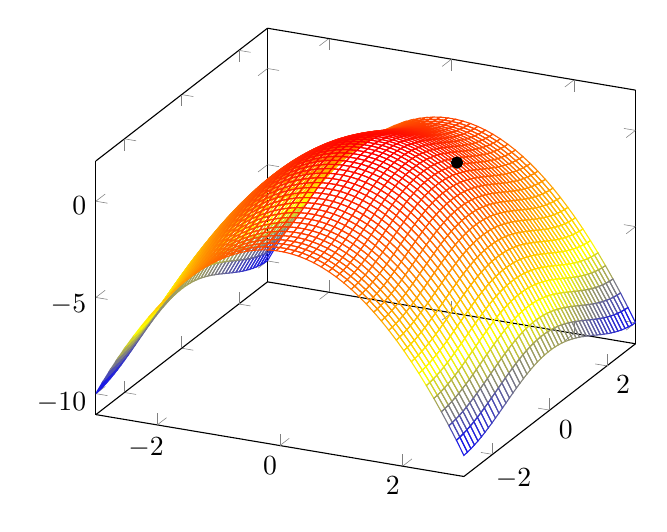
\begin{tikzpicture}
    \begin{axis}[]
        \addplot3[mesh, samples = 50, domain = -3:3]{cos(deg(y)) - x^2};
        \addplot3[black, mark=*] coordinates {(1, 1.047, -0.5)};
    \end{axis}
\end{tikzpicture}
    \caption{The surface $z = \cos{y} - x^2$}
    \label{fig:surface}
\end{figure}

We can see that $f(1, \pi/3) = -1/2$, therefore the point $(1, \pi/3, -1/2)$ 
lies on the surface $z = \cos{y} - x^2$ (the black dot shown in figure \ref{
fig:surface}). If we fix $y$ such that $y = \pi/3$, we are looking at the 
intersection between the surface and the plane $y = \pi/3$ (see figure \ref{
fig:tangent}). 

\begin{figure}[htbp]
    \centering
    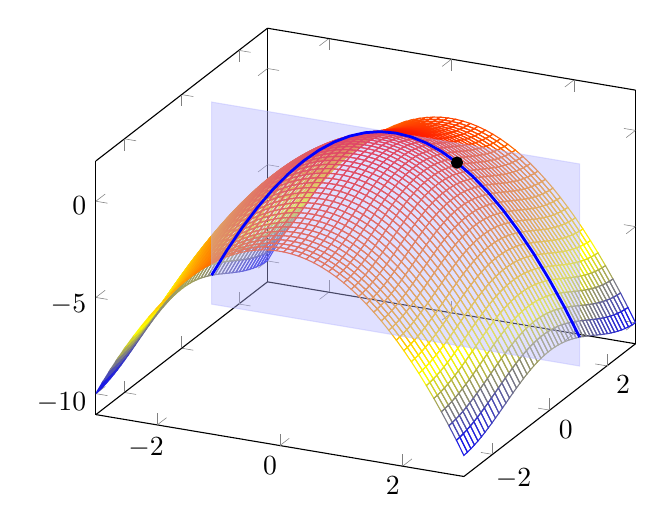
\begin{tikzpicture}
    \begin{axis}[]
        \addplot3[mesh, samples = 50, domain = -3:3]{cos(deg(y)) - x^2};
        \addplot3[black, mark=*] coordinates {(1, 1.047, -0.5)};
        \filldraw[blue!30, opacity = 0.4] (-3, 1.047, -10) -- (-3, 1.047, 0.5) 
        -- (3, 1.047, 0.5) -- (3, 1.047, -10) -- cycle;
        \addplot3+[draw=blue, line width = 1pt, domain = -3:3, samples y = 0, 
        mark=none] ({x}, 1.047, {0.5-x^2});
    \end{axis}
\end{tikzpicture}
    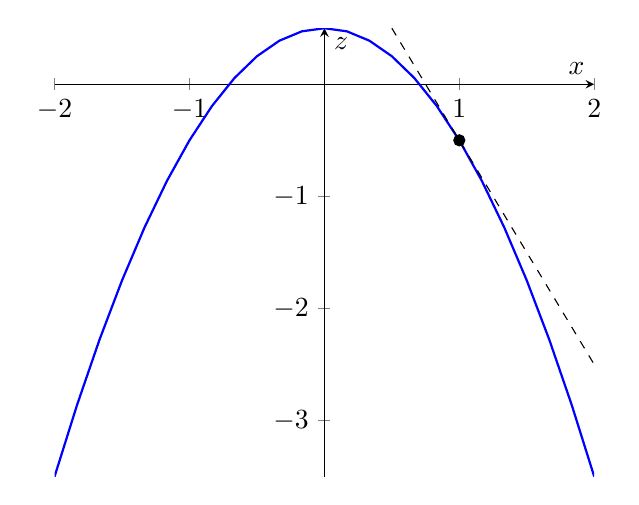
\begin{tikzpicture}
        \begin{axis}[axis lines = center, xlabel = $x$, ylabel = $z$]
            \addplot[blue, thick, domain = -2:2] {0.5-x^2};
            \addplot[black, thin, dashed, domain = 0.5:2] {-2*(x - 1) - 0.5};
            \addplot[black, mark=*] coordinates {(1, -0.5)};
        \end{axis}
    \end{tikzpicture}
    \caption{The intersection between the surface $z = \cos{y} - x^2$ and $y = 
    \pi/3$ is the parabola $z(x) = 1/2 - x^2$}
    \label{fig:tangent}
\end{figure}

We can describe this intersection as $g(x) = f(x, \pi/3)$, and therefore the 
slope of a tangent line to this intersection is given by $g'(x) = f_x(x, 
\pi/3)$. This means, geometrically, $f_x(1, \pi/3)$ is the slope of the line 
that lies tangent to $z = f(x, y)$ at the point $(1, \pi/3, -1/2)$ and in the 
plane $y = \pi/3$ (see figure \ref{fig:tangent}). Alternatively, you could 
think of $f_x$ as the slope of the tangent line to the surface that is 
parallel to the $x$-axis. 

\section{Gradient Vectors}

\section{Applications of Partial Derivatives and Gradients}

\subsection{Laplace's Equation}